% Source: graduate-coursework/Sp26/CSCE763/Course_Assignments/HW3/HW3_CSCE_763.tex

\documentclass[border=4pt]{standalone}
\usepackage{amsmath}
\usepackage{amssymb}
\usepackage{graphicx}
\usepackage{tikz}
\usepackage{xcolor}
\usetikzlibrary{shapes.geometric, arrows.meta, positioning, patterns}

\definecolor{USC_Garnet}{HTML}{73000A}
\definecolor{USC_Sandstorm}{HTML}{FFF2E3}
\definecolor{USC_Black90}{HTML}{363636}
\definecolor{USC_Black70}{HTML}{5C5C5C}
\definecolor{USC_Black50}{HTML}{A2A2A2}
\definecolor{USC_Black10}{HTML}{ECECEC}
\definecolor{USC_Honeycomb}{HTML}{65780B}
\definecolor{USC_Atlantic}{HTML}{466A9F}
\definecolor{USC_Congaree}{HTML}{1F414D}
\definecolor{USC_Rose}{HTML}{CC2E40}
\definecolor{outputbg}{RGB}{245,245,245}
\definecolor{tealfill}{HTML}{00B8A9}
\definecolor{teallight}{HTML}{D4F0ED}
\definecolor{lightblue}{HTML}{D6EAF8}

\begin{document}
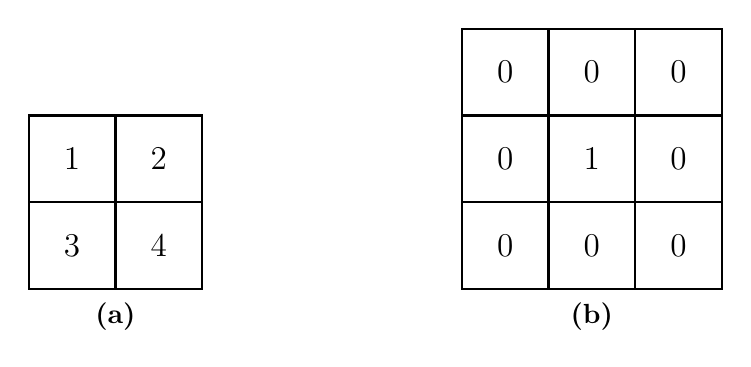
\begin{tikzpicture}[
  imgcell/.style={minimum size=1.1cm, draw=black, thick, fill=white, font=\large\bfseries},
  gridcell/.style={minimum size=1.1cm, draw=black, thick, fill=white, font=\large\bfseries},
]

% --- (a) 2x2 image ---
\node[imgcell] at (0, 1.1) {$1$};
\node[imgcell] at (1.1, 1.1) {$2$};
\node[imgcell] at (0, 0) {$3$};
\node[imgcell] at (1.1, 0) {$4$};
\node[font=\bfseries] at (0.55, -0.9) {(a)};

% --- (b) 3x3 identity image ---
\foreach \val/\col/\row in {
  0/0/2, 0/1/2, 0/2/2,
  0/0/1, 1/1/1, 0/2/1,
  0/0/0, 0/1/0, 0/2/0}
{
  \node[gridcell] at (5.5+\col*1.1, \row*1.1) {$\val$};
}
\node[font=\bfseries] at (6.6, -0.9) {(b)};

\end{tikzpicture}
\end{document}
